\section{Experiment 2}
\subsection{Methodology} \label{method-2}

%<---------------------------->%
% Motivation
%% The second experiment takes a step futher
%%% First: Mimics an HCI setting (generalization)
%%% Second: Different perspective
%%% Third: Different impact setting
%% We created a HCI scenerio and measure participant's preference using Likert, QV and a monetary task.
%<---------------------------->%

The first experiment results demonstrated strong implication that
QV aligns closer to participants true preference
compared to Likert scale 
when choosing among a sepctrum of societal issues.
To take a step futher, 
we designed the second experiment
with three different changes.
First, we changed the application domain form societal issues to an HCI application.
We examined QV's ability to generalize across different application domains.
Second, different from choosing among different societal causes that impacted the society as a whole,
the second experiment presented options that are different perspectives of the same subject matter.
This sutble difference lies in the different \textit{degree} that options relates to one another.
A simple analogy would be: 
if the first experiment asked about one's preference of ice cream flavors, 
the second experiment asked how much does one care about the texture, flavor and color of an ice cream.
Thrid, the second experiment produces a more immediate and concrete outcome 
rather than a more abstrat and further-in-the-future socieal impact.
We hypothesis that under these three conditions, QV will still outperform Likert 
at presenting subject's true preferences.
To test our hypothesis, we designed an 
between within subject study with two groups of participants.
Both group of participant were asked to walk through an HCI study
using different measuring techniques. 
In this section, we will explain the HCI study we designed, 
followed by the experiment workflow
accompanied with the reasoning of the experiment design.

%<---------------------------->%
% HCI Experiment background
%% Video HCI experiments
%% Selection of the five elements and their definitions
%% The goal of this HCI experiment is to find elements that impact participants most.
%<---------------------------->%
 
% The actual experiment, reason follows next
%% Two groups
%% Each group will follow path: demographic, ...
%% <img: experiment flow>
%%% explain each of the modules
%%% demographic
%%% learning and quiz
%%% sandbox
%%% <img: sandbox>
%%% buyback store
%%% <img: store>
%%% quiz on the video of buyback store
%%% <img: quiz>

% Why buyback 
% true preference: incentive compatiable
% this task pushes participants to be accurate

% Possible confounds and methods to offset these confounds.


\subsection{Choice of HCI study}
To prevent from coming up with an entire new HCI study that requires sophisticated verification,
We want a well-explored HCI topic that we could rely on to ensure ecological validity.
Most HCI research used Likert surveys to understand participant's opinions across one or more devices, designs, or interfaces.
%One could view this as one form of eliciting one out of $K$. 
However, reproducing one of these experiences can be costly and difficult because of the availability of these devices, designs, or interfaces.
Therefore, we turn to the other type of use case, where UX/UI researchers aimed to prioritize features and elements that their customers care about.
We see these forms often as online feedback forms.

Research on video and audio elements of video playback from the lens of HCI has been relatively mature.
Researchers provided insights to fields like multi-media conferencing \cite{watson1996evaluating}, video-audio perception \cite{chen2006cognitive, molnar2015assessing}and more specifically trade-offs between video and audio elements under network-monetary constraints \cite{molnar2013comedy, oeldorf2012bad}.
\textcite{oeldorf2012bad}, for example, conducted a study to understand how users with bandwidth constraints made trade-offs covering a broad set of elements across multiple video and audio elements. 
They examined participants' attitudes between three video bit rates, three video frame rates, and two audio sampling rates across three types of video content.
Participants were asked to rate the overall quality, video quality, audio quality, and enjoyment level on a 5-point Likert scale in each condition. 
The conclusion was drawn using the mean and standard deviation of the survey results.
%This is a typical study where the goal is to find one or some of the $K$ elements to choose from when under constraint.
We mimic this experiment and propose a similar user research scenario: 
Given limited bandwidth, how importand does participants think
the five video and audio elements were to a video watching experinece?
Based on related works, we elected the five video elements: (1) Stability of Video Imagery \cite{claypool1999effects}, (2) Stability of Audio \cite{claypool1999effects}, (3) Quality of audio \cite{oeldorf2012bad, noll1993wideband}, (4) Quality of the video \cite{oeldorf2012bad, knoche2008low}, and (5) Audio-Video Synchronization \cite{steinmetz1996human}. 
The ``Stability of Video Imagery'' refers to how smooth the visuals of the video plays. 
Lost packets during playback casues freezed frames. The more lost packets, the more staggered the video seems.
The ``Stability of Audio'' is similiar of video, which refers to the smoothness the audio is. Lost audio packets creates silence, causing the audio to stutter. 
The ``Quality of audio'' refers to how clear and crisp the sound quality are of the video.
With a lower audio sampling rate,
a smaller audio file is required, vice cersa.
The lower the audio quality, the more muffled and unclear the audio aounds.
Similiar to audio quality, the ``Quality of the video'' refers to how sharp the visuals in the video are.
Resolutions are proportion to the number of pixels sent to the client from the server. Hence, by altering the length and width of the video, or pixel density per inch, we change the quality and size of the video file. The smaller the pixels,
the more pixelated and unclear the video seems.
Finally, the ``Video-audio Synchronization'' is how well video visuals synchronized with the audio playback.
In our experiment, we focus on having audio play ahead of the video only.
Since there are no previous studies that looked at the combination of all these video elements, we make use of indiviual studies to create the various levels of changes used in this experiment.
In short, we make use of a video-audio experiment as the research scenerio that we want to test Likert and QV.
This video-audio experiment aims at finding video/audio elements that impact participants the most.

\begin{figure}[htpb]
    \centering
    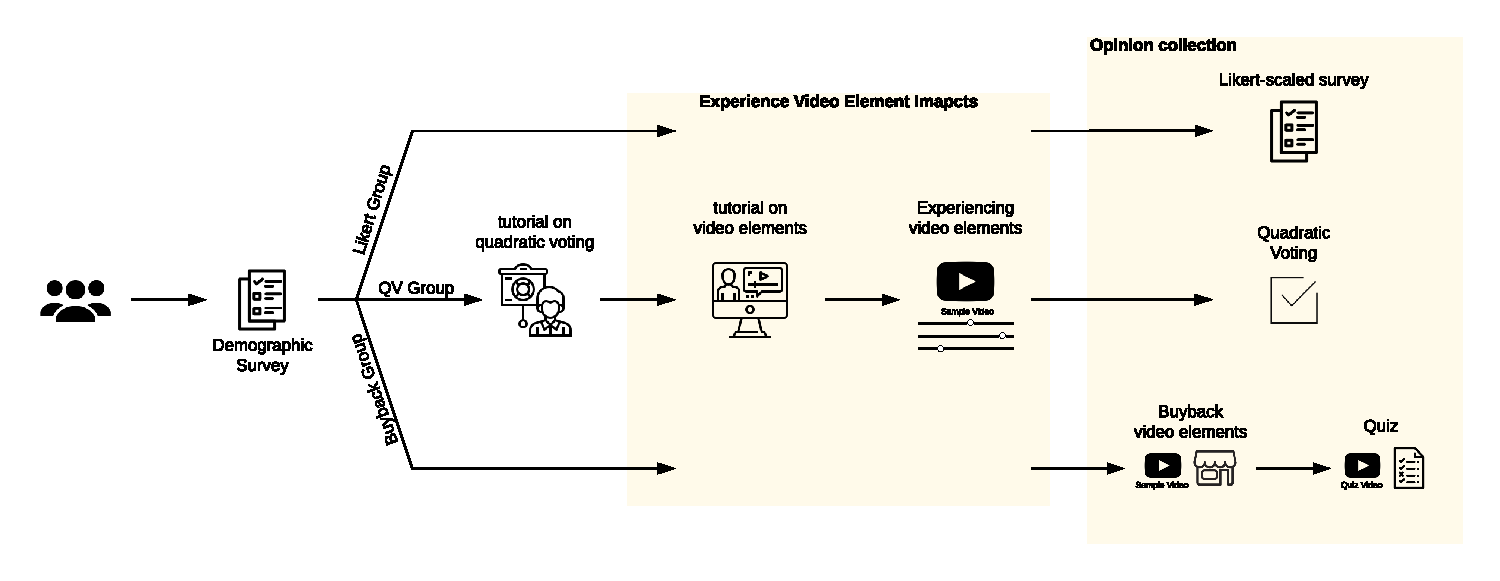
\includegraphics[width=\textwidth, keepaspectratio=true]{content/image/exp2_flow.pdf}
    \caption{
        Experiment two was conducted between subjects. Participants were divided into three groups. Participants that took the first path are the Likert Group, the center path is the QV group, and the bottom path is the buyback Group. The first two groups of participants expressed their opinions of various video elements in terms of a five-point Likert scale or a 100-credit QV. The third group will complete a ``buyback'' task that purchases video elements that they believe will assist them in completing a quiz.
    }
    \label{fig:exp2_flow}
\end{figure}

We recruited 180 participants through MTurk.
To compare how Likert survey and QV reflects people's underlying preferences,
we desgined the following experiment structure.
All participants will follow these five steps, the shaded area in Figure \ref{fig:exp2_flow} in sequence, starting with (1) Demographics, (2) Learning and attention checks, (3) Video Playground, (4) Expressing attitude, and finally the (5) Buyback Task.
Participants were divided participants into two equal groups: Likert and QV. 
The two groups differ by how they reveal their attidutes in step four;
Likert group responding with a Likert survey and QV group express using QV.
%This experiment also acts as a concrete example of how QV can be incorporated in HCI.

The experiment starts with a demographic survey, identical to the first experiment.
In the second step, we provided participants with tutorials on the definition of video elements. Participants then complete a quiz containing five mutiple choice questions for us to make sure they fully understood the content.
Given QV unpopular among the mass, we added an additional tutorial on QV and attention checks specific to QV for the QV Group.

Once participants passed the attention checks, we provide them a playground that allows hands-on experience on how different video elements impact their viewing experiencs. We describe this further in the next subsection. Participants can interact with this experience as long as they like. %TODO: Participants were told that this research is conducted by a video streaming company primarily serving in-flight entertainment systems.
% During flights, data bandwidth is limited and engineers of the company need to know what to prioritize to serve the customer.
% We believe this scenario is easy to understand and can be easily applied to many real-life situations, such as a sudden drop in a mobile network, spotty WiFi connection, or unstable inflight internet.
% We also believe that participants have experience degrade in at least one of the five video elements in the past, making this task easy to understand and relay.

After participants moved on, we ask participants to provide how important they think each of the five video elements were to their viewing experience. The Likert Group used a five-point likert scale survey. The QV group used the QV interface similiar to that of the first experiment. The only difference compared with Figure \ref{fig:system_interface} is that instead of societal casues, we list the five video elements as options. With results from experiment 1, we provided participants each with 100 voice credits.

Participants then end the experiment by conducting a task -- buyback task -- as the respresentation of their underlying true preferences. We describe the buyback task in depth in subsection KK.


\subsection{Video Playground}
Recall participants were provided the scenerio that we were an online streaming company trying to understand how they value these differernt video elements.
We want participants to experience and understand how different video elements impact a video
and therefore we built the video playgorund interface, shown in Fig %\ref{fig:exp2_flow}.

This interface showcased a weather video on top of the page.
For each of the five video elements,
we provided one control with four levels of toggles.
Participants can toggle any of these five elements to any of the four toggles at any time.
According to the toggles, the interface presentes immediate changes to the weather video.
Participants can pause and play the video at any time and they can reply the video as many times as they like.
We list the four levels of each toggle in table M. 
Each of these levels were selected based on previous studies and designed to be as linear to the user's perception as possible. 

In addition to the toggles, we added five mutiple choice questions at the bottom of the same page. These questions asked factual questions based on the content of the video. We told participants that their response would be invalidated if they answer two or more multiple choice questions incorrectly. These questions can make sure pariticpants completely finished watching the video at least once. Further, these questions primed all participants in the experiment with the same goal of understanding the video context and not just for pure entertainment purposes.


% \begin{figure}[htpb]
%     \centering
%     \includegraphics[width=\textwidth, keepaspectratio=true]{resources/exp_2_video.png}
%     \caption{
%         Real-time Video Element Interface
%     }
%     \label{fig:exp_2_video}
% \end{figure}


\subsection{Buyback task}
It is non-trival, compared to the donation task in the previous experiment, to measure a participant's real preference on video elements. We designed \textbf{the buyback task} to capture this preference. Participants were told the possiblity of earning extra bonus during this task.

Therefore, we created a ``video element store'' that allows participants to buy video elements. This buyback store is presented in Figure J. Participants were now given the same weather video that mimics the worst-case scenarios under limited internet bandwidth, where each of the five video elements set to level 0. 

We told participants that they could ``enhance'' each of these elements by``spending'' on each of these elements becasue they will use the combination they purchased to complete the next task. Participants will answer five factual questions on a different weather video applied with this set of element settings. If participants answer 80\% of five multiple-choice questions correctly, they will enter a lottery that pays the winner their own remaining amount from what they purchased. For example, if the winning participant spent 40 dollars and answered four out of the five questions correctly, they will win 10 dollars becasue their total budget is 50 dollars. This provides an incentive-compatiable setting to the participants. Participants, assuming being rational, will find a balance for each of the elements as their willingness to pay (WTP). This setting is somewhat common in real life where many subscription-based services on the market requires customers pay additional premiums for additional benefits. Another example are gamers making purchases in stores that equip online avatars with extra features to compete with other gamers in online games.
%With tasks in hand, participants will considering the best use of their budget but understanding the content in the video.The Quiz ensures that participants have correctly comprehended the video.

Let us explain the deatils of this experiment. First we examin the buyback store. Having the layout similiar to the video playground, the major difference lies in the control panel. We changed the control for each of the five element into a slider without ticks. These sliders were accompanied by a text input box to the right. Participants can pull the slider to anywhere and the system would reflect the reletive position of the slider between 0 and 10, representing the 10 dollars. Alternatively, participants can put in a value between 0 and 10 and the slider will move to the corresponding location.

When the slider moves, the video above still reflects immediatly of the setting.
However, participants are not aware of \textbf{how many} and \textbf{where} levels exist in this control panel. The interface will automatically translate the input value (between 0 and 10) into nine different levels presented in table O. 
There are several considerations for this design. 
One consideration is that by hidding the number of levels present, participants now has the freedom to put in any value that they ``believe'' they want to devote. Participants are not constrained by the ``ticks'' we presented since they do not know ``where'' each level changes, making their input value truthful. Another consideration is that we based the nine levels on the four levels presented in the video playground. This means that we are not altering participants previous experience, but allow them to experience and purchase more fine grain features. The last consideration is we choose these levels based on a pilot and assure participants can accomplish the tasks without spending all their budgets. We detail this pilot in the appendix.

The second detail is in the quiz page of the buyback. On this page, participants can replay the video as many times as they want with the five factual multiple choice questions on the same page. This means participants do not need to memorize the content of the video. We ask participants questions like "What is the weather of Chicago?", "What is the highs and lows of San Diego," and "Which city was not shown in the video?". These questions are similiar to the ones we presented in the video playground. We also list these questions in text form to assist participants in making their purchase decisions. 

%To the best of our knowledge, we are the first to design such a task, yet, it reflects many behaviors in real life.